\chapter{The Large Hadron Collider}
%\section{Siliziumdetektoren}
The LHC was build between 1998 and 2008 by the European Organization for Nuclear Research (CERN) in collaboration with 10000 scientist from over 100 countries
and lies in a $\SI{27}{\kilo\meter}$ tunnel 175 metres underground in Switzerland near Geneva. It is a proton-proton synchrotron, which uses
the systems to accelerate the protons before they are injected into the main accelerator. The linear particle accelerator LINAC 4 generates $\SI{160}{\mega\eV}$
negative hydrogen ions and launches them into the Proton Synchrotron Booster (PSB). Here, the electrons are removed from the hydrogen ions, leaving only the nucleus
consisting of one proton, which then enters the Super Proton Synchrotron (SPS). It increases the protons energy to $\SI{450}{\GeV}$ and feeds them to the
LHC, where to opposing proton beams are accelerated. In the main ring,
the protons are accumulated to bunches and accelerated to their maximum energy of $\SI{13}{\tera\eV}$ in 20 minutes.

At four locations, the two proton beams
are crossed, making it possible for them to collide. Around these interaction points, the four large experiments, ATLAS, CMS, LHCb and Alice are operated.
Occasionaly lead nuclei are accelerated to study matter under extreme conditions at the ALICE experiment. The ATLAS and CMS experiment are general-purpose detectors for
high energy physics. They differ on their technical design to achieve their goal and enable to corrobate each others results.
LHCb is an asymmetric particle detector specialized in measuring the parameters of CP violation in B-meson decays.
Further experiments at the LHC include TOTem, LHCf, MoEDAL and FASER, which focus on specialized research. Figure \ref{fig:lhc_aufbau} shows the schematic depiction
of the LHC.

\begin{figure}[H]
  \centering
  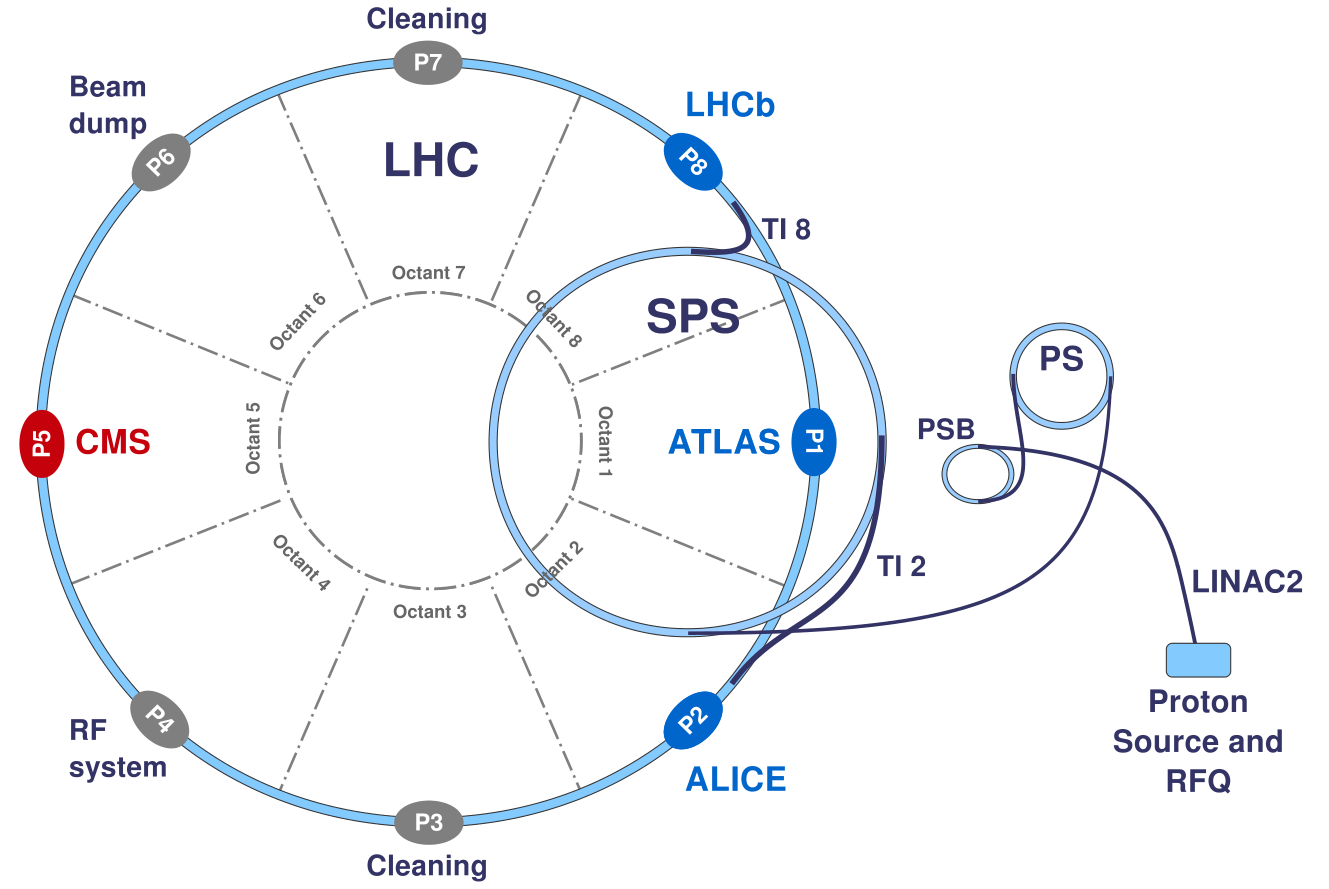
\includegraphics[height=0.4\textwidth]{images/lhc_aufbau.png}
  \caption{Schematic representation of the CERN accelerator complex (not to scale)\cite{lhc_aufbau}.}
  \label{fig:lhc_aufbau}
\end{figure}

After the second run from 2015 to 2018 followed the Long Shutdown 2 (LS2) until 2021 in order to upgrade the accelerator. The goal is to increase the luminosity by a factor of 10 by
implementing High Luminosity Large Hadron Collider (HL-LHC) in the Long Shutdown 3 (LS3), which is planned to be operational in 2026. Figure \ref{fig:lhc_plan} shows the timeline
of LHC programme.

\begin{figure}
  \centering
  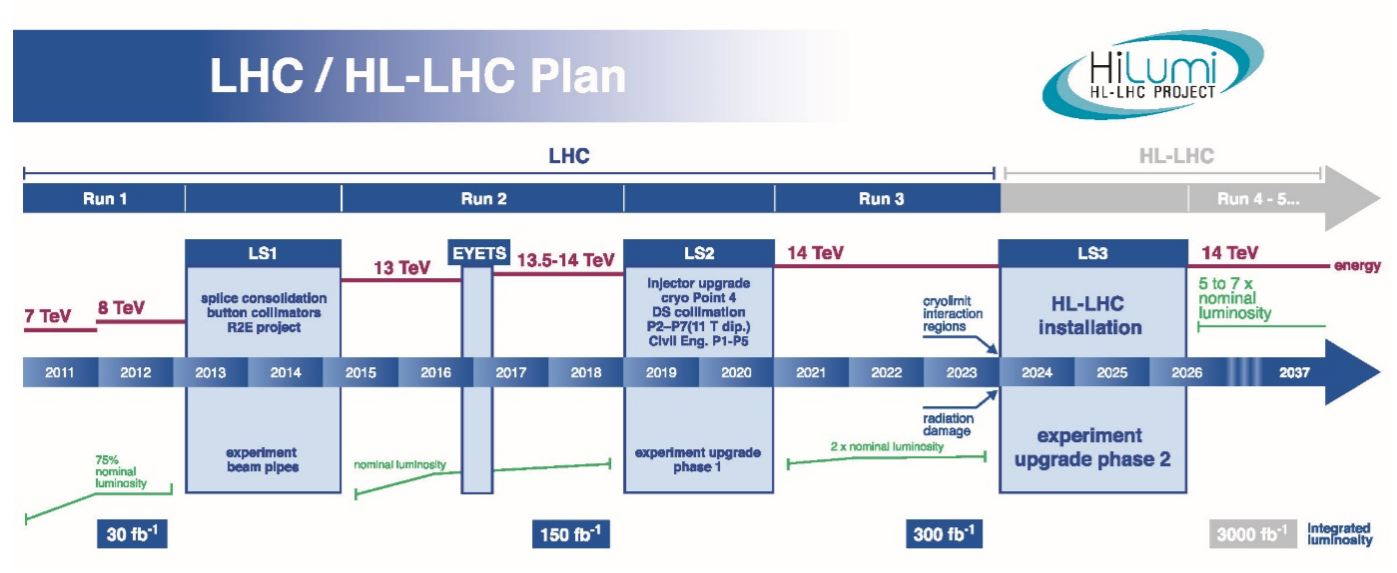
\includegraphics[height=0.4\textwidth]{images/lhc_plan.png}
  \caption{Timeline of the operational phases and Shutdowns of the LHC. The energy of accelerated protons in each phase is shown in red and the luminosity in green \cite{lhc_plan}.}
  \label{fig:lhc_plan}
\end{figure}
